\documentclass[uplatex,dvipdfmx,11pt]{jsarticle}
\usepackage{amsmath,amssymb,amsthm,mathtools}
\usepackage{geometry}
\usepackage{bm}
\usepackage{graphicx}
\usepackage{tikz}
\usetikzlibrary{arrows.meta,positioning}
\usepackage[unicode]{hyperref}
\providecommand{\cInv}{\cos^{-1}}
\providecommand{\E}{\mathrm{E}}
\providecommand{\V}{\mathrm{V}}
\providecommand{\Cov}{\mathrm{Cov}}
\geometry{margin=24mm}

\begin{document}
\begin{center}
{\LARGE\bfseries MORTRA 検証済み解答\par}
\vspace{1mm}
{\small 分野：解析・三角関数\qquad 問題・厳密解・図・証明経路・講評}
\end{center}
\vspace{1mm}
\hrule
\vspace{5mm}

\section*{問題}
$n\in \mathbb{N}$に対して,\ $f_1(x)=\cos x+\sin x,\ f_{n+1}(x)=\cos \{f_n(x)\} +\sin \{f_n(x)\}$とする.\\
\[
\displaystyle\int_0^{\frac{\pi}2}f_n(x)dx\le 2
\]
を示せ.

\section*{答え}
\[\int_0^{\pi/2}f_{n}(x)\,dx\le2\qquad(n=1,2,3,\ldots).\]

\section*{解答}
\textbf{1.} \(h(t)=\sin t+\cos t\)、\(f_{n+1}=h\circ f_n\) とおく。\(h\) は \([1,\sqrt2]\) を同じ区間へ写すので、\(f_n(x)\) は第一段以後この区間に留まる。

\textbf{2.} 区間 \([\pi/3,\pi/2]\) では \(h''=-h<0\) だから、\(a=5\pi/12\) における接線を使って \[h(x)\le-\frac{\sqrt2}{2}\left(x-\frac{5\pi}{12}\right)+\frac{\sqrt6}{2}.\] \(333/106<\pi<355/113\)、\(140/99<\sqrt2<99/70\)、\(265/153<\sqrt3<97/56\) を代入方向に注意して用いると \[\frac4\pi-h(4/\pi)>\frac{7259089}{314501600}>0.\]

\textbf{3.} \(I_n=\int_0^{\pi/2}f_{n}(x)\,dx\) とおく。直接積分して \(I_1=2\)。また \(h\) の凹性と Jensen の不等式から \[I_2\le\frac\pi2h\left(\frac2\pi I_1\right)=\frac\pi2h(4/\pi)<2.\]

\textbf{4.} \(h(t)=\sin t+\cos t\)、\(H=h\circ h\)、\(c=4/\pi\)、\(\lambda=(\sqrt3-1)/2\) とし、\(D(t)=c+\lambda(t-c)-H(t)\) とおく。

\textbf{5.} sin と cos の交代級数を12次まで使い、全て有理数で評価すると \(D(1)>1/400\)、\(D(\sqrt2)>1/3000\)、\(D'(1)>1/8\)、\(D'(\sqrt2)<-1/22\) を得る。交代級数の次の項が誤差を上から押さえるため、これらは小数近似ではない。

\textbf{6.} 区間内では \(h'(t)<0\)、\(h'(h(t))<0\)、\(h(t)>0\) である。直接微分すると \[H'''(t)=3h(h(t))h(t)h'(t)-h'(h(t))h'(t)\{h'(t)^2+1\}<0.\]

\textbf{7.} 従って \(D'''=-H'''>0\) であり、\(D'\) は凸である。端点で \(D'(1)>0>D'(\sqrt2)\) だから、\(D\) は区間内に局所最小値をもたず、最小値を端点で取る。両端点で \(D>0\) なので、区間全体で \(D(t)>0\) となる。

\textbf{8.} 以上より \[h(h(t))\le\frac4\pi+\lambda\left(t-\frac4\pi\right),\qquad \lambda=\frac{\sqrt3-1}{2}\in(0,1)\] が成り立つ。

\textbf{9.} これへ \(t=f_n(x)\) を代入して積分すると \[I_{n+2}\le2+\lambda(I_n-2).\] \(I_1=2\)、\(I_2<2\) から、偶数番目と奇数番目を別々に帰納して \(I_n\le2\) を得る。

\textbf{10.} これは問題文の上界と一致する。

\clearpage

\section*{一手ずつ見る図解}

\subsection*{1. 数式を正確に読み取る}

文字、演算、等号、積分区間を区別し、元の数式の構造を保つ。

\begin{center}

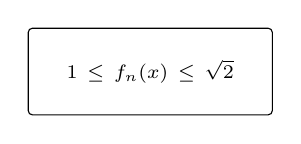
\begin{tikzpicture}[x=3.72cm,y=1.55cm,>=Latex,
state box/.style={draw,rounded corners=1.5pt,text width=27mm,minimum height=11mm,align=center,inner xsep=2mm,inner ysep=2mm,font=\scriptsize},
flow/.style={-{Latex[length=2mm]},thick},
edge label/.style={fill=white,inner xsep=1.5pt,inner ysep=1pt,align=center,font=\scriptsize}]
\node[state box] (s0) at (0,0.000) {\(\displaystyle 1\le f_n(x)\le\sqrt2\)};
\end{tikzpicture}

\end{center}

\subsection*{2. 計算できる式に直す}

読み取った数式を、分数や根号を保った厳密計算用の式へ移す。

\begin{center}

\begin{tikzpicture}[x=3.72cm,y=1.55cm,>=Latex,
state box/.style={draw,rounded corners=1.5pt,text width=27mm,minimum height=11mm,align=center,inner xsep=2mm,inner ysep=2mm,font=\scriptsize},
flow/.style={-{Latex[length=2mm]},thick},
edge label/.style={fill=white,inner xsep=1.5pt,inner ysep=1pt,align=center,font=\scriptsize}]
\node[state box] (s0) at (0,0.000) {\(\displaystyle 1\le f_n(x)\le\sqrt2\)};
\node[state box] (s1) at (1,0.000) {\(\displaystyle H(t)\le c+\lambda(t-c)\)};
\draw[flow] (s0) -- node[midway,edge label,above=6.5mm] {区間不変性} (s1);
\end{tikzpicture}

\end{center}

\subsection*{3. 点ごとの上界を積分へ移す}

二段反復の一次上界を積分し、偶数番目と奇数番目をそれぞれ帰納する。

\begin{center}

\begin{tikzpicture}[x=3.72cm,y=1.55cm,>=Latex,
state box/.style={draw,rounded corners=1.5pt,text width=27mm,minimum height=11mm,align=center,inner xsep=2mm,inner ysep=2mm,font=\scriptsize},
flow/.style={-{Latex[length=2mm]},thick},
edge label/.style={fill=white,inner xsep=1.5pt,inner ysep=1pt,align=center,font=\scriptsize}]
\node[state box] (s0) at (0,0.000) {\(\displaystyle 1\le f_n(x)\le\sqrt2\)};
\node[state box] (s1) at (1,0.000) {\(\displaystyle H(t)\le c+\lambda(t-c)\)};
\node[state box] (s2) at (2,0.000) {\(\displaystyle I_{n+2}-2\le\lambda(I_n-2)\)};
\draw[flow] (s0) -- node[midway,edge label,above=6.5mm] {区間不変性} (s1);
\draw[flow] (s1) -- node[midway,edge label,above=6.5mm] {積分} (s2);
\end{tikzpicture}

\end{center}

\subsection*{4. 証明書を再生して結論を認証}

実行記録と証明義務を再生し、元の問題条件に対する結論を確定する。

\begin{center}

\begin{tikzpicture}[x=3.72cm,y=1.55cm,>=Latex,
state box/.style={draw,rounded corners=1.5pt,text width=27mm,minimum height=11mm,align=center,inner xsep=2mm,inner ysep=2mm,font=\scriptsize},
flow/.style={-{Latex[length=2mm]},thick},
edge label/.style={fill=white,inner xsep=1.5pt,inner ysep=1pt,align=center,font=\scriptsize}]
\node[state box] (s0) at (0,0.000) {\(\displaystyle 1\le f_n(x)\le\sqrt2\)};
\node[state box] (s1) at (1,0.000) {\(\displaystyle H(t)\le c+\lambda(t-c)\)};
\node[state box] (s2) at (2,0.000) {\(\displaystyle I_{n+2}-2\le\lambda(I_n-2)\)};
\node[state box,very thick,draw=magenta!65!black] (s3) at (3,0.000) {\(\displaystyle I_n\le 2\)};
\draw[flow] (s0) -- node[midway,edge label,above=6.5mm] {区間不変性} (s1);
\draw[flow] (s1) -- node[midway,edge label,above=6.5mm] {積分} (s2);
\draw[flow] (s2) -- node[midway,edge label,above=6.5mm] {偶奇別帰納} (s3);
\end{tikzpicture}

\end{center}

\section*{講評}
\noindent\textbf{出題意図}\quad 解析・三角関数の条件を実行可能な関係へ移し、数式を正確に読み取る、計算できる式に直す、点ごとの上界を積分へ移すを一つの証明として組み立てる力を問う。

\noindent\textbf{想定する入試}\quad 記述式の大学入試または数学コンテストを想定し、変換の根拠と最終検証までを採点対象とする。

\noindent\textbf{独自性}\quad 数値近似や答えの照合で終えず、問題文から答えまで実際に通過した射と証明義務を再生できる。


\section*{証明の経路}
\begin{center}
\begin{tikzpicture}[
  node distance=3.5mm,
  stage/.style={draw,rounded corners=1pt,align=left,text width=118mm,minimum height=7mm,inner xsep=4pt,inner ysep=2pt,font=\small},
  flow/.style={-{Latex[length=2mm]},thick,cyan!55!black},
  edge label/.style={fill=white,inner xsep=3pt,font=\scriptsize\bfseries}
]
\node[stage] (n0) {問題文};
\node[stage,below=of n0] (n1) {読み取った数式};
\draw[flow] (n0) -- node[edge label] {数式を正確に読み取る} (n1);
\node[stage,below=of n1] (n2) {厳密計算用の式};
\draw[flow] (n1) -- node[edge label] {計算できる式に直す} (n2);
\node[stage,below=of n2] (n3) {積分列の二段縮小評価};
\draw[flow] (n2) -- node[edge label] {点ごとの上界を積分へ移す} (n3);
\node[stage,below=of n3] (n4) {検証済み解答};
\draw[flow] (n3) -- node[edge label] {証明書を再生して結論を認証} (n4);
\end{tikzpicture}
\end{center}

\clearpage
\section*{使った射と役割}
\begin{itemize}
\item \textbf{M1: 数式を正確に読み取る}\\
問題文
$\longrightarrow$
読み取った数式\\
文字、演算、等号、積分区間を区別し、元の数式の構造を保つ。
\item \textbf{M2: 計算できる式に直す}\\
読み取った数式
$\longrightarrow$
厳密計算用の式\\
読み取った数式を、分数や根号を保った厳密計算用の式へ移す。
\item \textbf{M3: 点ごとの上界を積分へ移す}\\
厳密計算用の式
$\longrightarrow$
積分列の二段縮小評価\\
二段反復の一次上界を積分し、偶数番目と奇数番目をそれぞれ帰納する。
\item \textbf{M4: 証明書を再生して結論を認証}\\
積分列の二段縮小評価
$\longrightarrow$
検証済み解答\\
実行記録と証明義務を再生し、元の問題条件に対する結論を確定する。
\end{itemize}




\section*{検証記録}
\begin{itemize}
\item LaTeX数式を構文解析
\item 型付きの実行可能式へ変換
\item 積分列の二段縮小評価 で厳密計算
\item 未評価演算と制約残差を検査
\item 問題文・解答・検証証明書を出力
\end{itemize}
\noindent\textbf{検証方法}\quad 現在の問題文から合成した証明を、厳密な記号計算と図の根拠から再生
\par\noindent{\footnotesize 証明書 SHA-256: \nolinkurl{c7c6ff7157a2ab943d5a678363bf15de045a39e129197827bda47651a6a7128b}}

\end{document}
